%%%%%%%%%%%%%%%%%%%%%%%%%%%%%%%%%%%%%%%%%%%%%%%%%%%%%%%%%%%%%%%%%%%%%%
%%                     Stimulation
%%%%%%%%%%%%%%%%%%%%%%%%%%%%%%%%%%%%%%%%%%%%%%%%%%%%%%%%%%%%%%%%%%%%%%

\subsection{Glyph: \glyph{Stimulation}}\label{sec:stimulation}

A stimulation affects \textbf{positively} the flux of a process represented by the target process. This stimulation can be for instance a catalysis or a positive allosteric regulation. Note that \glyph{catalysis} exists independently in SBGN, see \sect{catalysis}. The target extremity of a \glyph{stimulation} carries an empty arrowhead.

\begin{figure}[H]
  \centering
  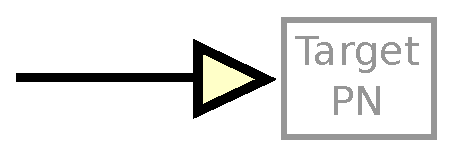
\includegraphics[scale = 0.5]{images/stimulation}
  \caption{The \PD glyph for \glyph{stimulation}.}
  \label{fig:stimulation}
\end{figure}

The example in \fig{stimulation-reversible} illustrates the use of two \glyph{stimulations} arcs to represent the opposite effects of agonists and inverse agonists on G-protein coupled receptor activity. Agonists stimulate the transition from inactive to active, while inverse agonists stimulate the transition inactive to active.

\begin{figure}[H]
  \centering
  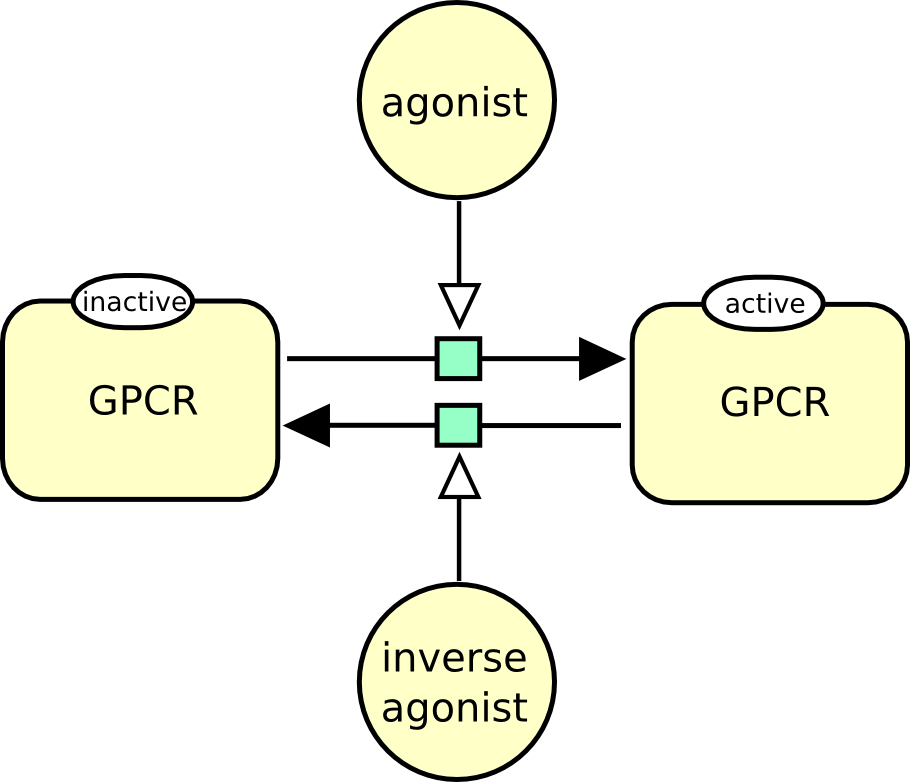
\includegraphics[scale = 0.5]{images/stimulation-reversible}
  \caption{Opposite effects of agonists and inverse agonists on GPCRs.}
  \label{fig:stimulation-reversible}
\end{figure}
